\documentclass[tikz,border=8pt]{standalone}
\usepackage{amsmath}
\usetikzlibrary{arrows.meta,positioning}

\begin{document}
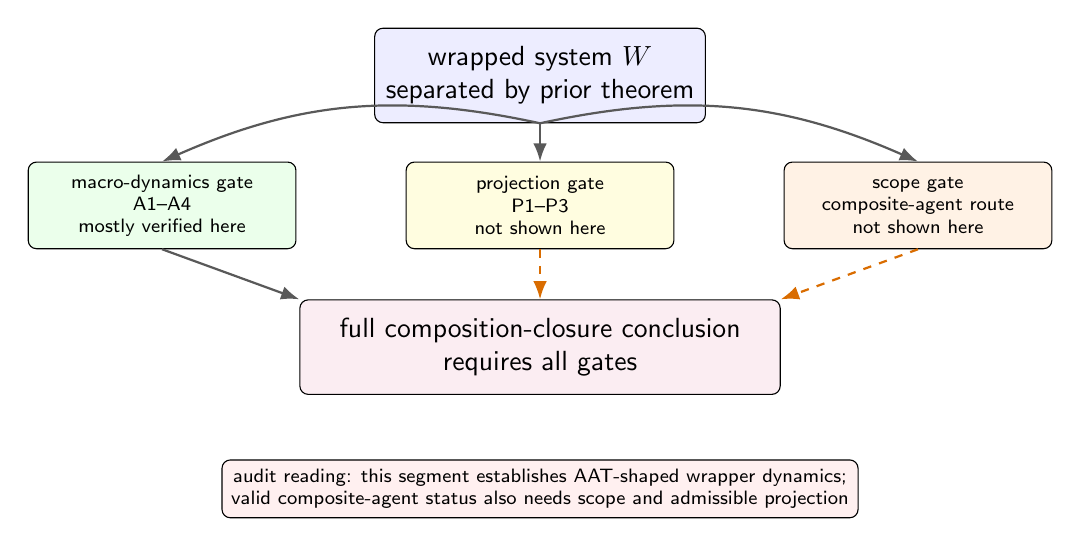
\begin{tikzpicture}[
  font=\sffamily,
  box/.style={draw, rounded corners=3pt, align=center, minimum width=42mm, minimum height=12mm, fill=white},
  gate/.style={draw, rounded corners=3pt, align=center, font=\sffamily\scriptsize, minimum width=34mm, minimum height=11mm, fill=white},
  note/.style={draw, rounded corners=3pt, align=center, font=\sffamily\scriptsize, fill=white},
  arrow/.style={-Latex, thick, draw=black!65},
  warn/.style={-Latex, thick, dashed, draw=orange!85!black}
]

\node[box, fill=blue!7] (wrapper) at (0,2.4)
  {wrapped system $W$\\separated by prior theorem};

\node[gate, fill=green!8] (macro) at (-4.8,0.75)
  {macro-dynamics gate\\A1--A4\\mostly verified here};
\node[gate, fill=yellow!12] (proj) at (0,0.75)
  {projection gate\\P1--P3\\not shown here};
\node[gate, fill=orange!10] (scope) at (4.8,0.75)
  {scope gate\\composite-agent route\\not shown here};

\draw[arrow] (wrapper.south) to[bend right=18] (macro.north);
\draw[arrow] (wrapper.south) -- (proj.north);
\draw[arrow] (wrapper.south) to[bend left=18] (scope.north);

\node[box, fill=purple!7, minimum width=61mm] (claim) at (0,-1.05)
  {full composition-closure conclusion\\requires all gates};
\draw[arrow] (macro.south) -- (claim.north west);
\draw[warn] (proj.south) -- (claim.north);
\draw[warn] (scope.south) -- (claim.north east);

\node[note, fill=red!6, minimum width=72mm] at (0,-2.85)
  {audit reading: this segment establishes AAT-shaped wrapper dynamics;\\valid composite-agent status also needs scope and admissible projection};

\end{tikzpicture}
\end{document}
